\begin{exo}
	Les points suivants $R\coordl{2}{1}$, $S\coordl{9}{3}$ et $T\coordl{13}{4}$ sont-ils alignés ? Justifier.

	\begin{center}
		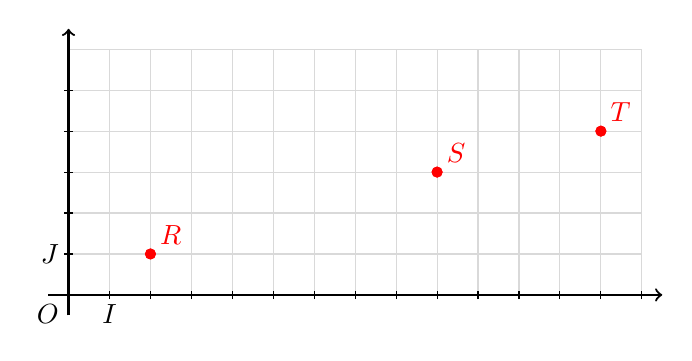
\begin{tikzpicture}[scale=0.52]
			\draw[gray!30, thin] (0,0) grid (14,6);
			\draw[thick,->] (-0.5,0) -- (14.5,0);
			\draw[thick,->] (0,-0.5) -- (0,6.5);
			\node at (0,0) [below left] {$O$};
			\node at (1,0) [below] {$I$};
			\node at (0,1) [left] {$J$};
			\foreach \x in {1,2,...,14} { \draw (\x, -0.1) -- (\x, 0.1); }
			\foreach \y in {1,2,3,4,5} { \draw (-0.1,\y) -- (0.1,\y); }
			\coordinate (R) at (2,1);
			\coordinate (S) at (9,3);
			\coordinate (T) at (13,4);
			\foreach \p/\name in {R/R, S/S, T/T} {
					\filldraw[red, thick] (\p) circle (3pt);
					\filldraw[red, thick] (\p) circle (3pt);
					\node[above right, red] at (\p) {$\name$};
				}
		\end{tikzpicture}
	\end{center}
\end{exo}
